\documentclass[conference]{IEEEtran}
\IEEEoverridecommandlockouts
% The preceding line is only needed to identify funding in the first footnote. If that is unneeded, please comment it out.
\usepackage{cite}
\usepackage{amsmath,amssymb,amsfonts}
\usepackage{algorithmic}
\usepackage{graphicx}
\graphicspath{{Imgs/}}
\usepackage{textcomp}
\usepackage{xcolor}
\usepackage{hyperref}
\usepackage{multicol}
\usepackage{listings}
\usepackage{color}
\lstloadlanguages{C,C++,csh,Java}

\definecolor{red}{rgb}{0.6,0,0} 
\definecolor{blue}{rgb}{0,0,0.6}
\definecolor{green}{rgb}{0,0.8,0}
\definecolor{cyan}{rgb}{0.0,0.6,0.6}

\lstset{
language=csh,
basicstyle=\footnotesize\ttfamily,
numbers=left,
numberstyle=\tiny,
numbersep=5pt,
tabsize=2,
extendedchars=true,
breaklines=true,
frame=b,
stringstyle=\color{blue}\ttfamily,
showspaces=false,
showtabs=false,
xleftmargin=17pt,
framexleftmargin=17pt,
framexrightmargin=5pt,
framexbottommargin=4pt,
commentstyle=\color{green},
morecomment=[l]{//}, %use comment-line-style!
morecomment=[s]{/*}{*/}, %for multiline comments
showstringspaces=false,
morekeywords={ abstract, event, new, struct,
as, explicit, null, switch,
base, extern, object, this,
bool, false, operator, throw,
break, finally, out, true,
byte, fixed, override, try,
case, float, params, typeof,
catch, for, private, uint,
char, foreach, protected, ulong,
checked, goto, public, unchecked,
class, if, readonly, unsafe,
const, implicit, ref, ushort,
continue, in, return, using,
decimal, int, sbyte, virtual,
default, interface, sealed, volatile,
delegate, internal, short, void,
do, is, sizeof, while,
double, lock, stackalloc,
else, long, static,
enum, namespace, string},
keywordstyle=\color{cyan},
identifierstyle=\color{red},
backgroundcolor=\color{cloudwhite},
}
\usepackage{caption}
\DeclareCaptionFont{white}{\color{white}}
\DeclareCaptionFormat{listing}{\colorbox{blue}{\parbox{\textwidth}{\hspace{15pt}#1#2#3}}}
\captionsetup[lstlisting]{format=listing,labelfont=white,textfont=white, singlelinecheck=false, margin=0pt, font={bf,footnotesize}}
\definecolor{cloudwhite}{rgb}{0.9412, 0.9608, 0.8471} 




\renewcommand{\abstractname}{Abstracto}
\def\BibTeX{{\rm B\kern-.05em{\sc i\kern-.025em b}\kern-.08em
    T\kern-.1667em\lower.7ex\hbox{E}\kern-.125emX}}
\begin{document}
\renewcommand\IEEEkeywordsname{Palabras clave}

{\footnotesize 
\title{Ensamblador y simulador de microprocesador basado en el Intel 8086.}
}

\author{
\IEEEauthorblockN{García García Jonathan Eduardo}
\IEEEauthorblockA{\href{mailto:jgarciag1404@alumno.ipn.mx}{jgarciag1404@alumno.ipn.mx}}
\and
\IEEEauthorblockN{González Santiesteban Santiago}
\IEEEauthorblockA{\href{mailto:sgonzalezs1400@alumno.ipn.mx}{sgonzalezs1400@alumno.ipn.mx}}
\and
\IEEEauthorblockN{Guzmán Olvera Jessica}
\IEEEauthorblockA{\href{mailto:jguzmano1701@alumno.ipn.mx}{jguzmano1701@alumno.ipn.mx}}
}

\maketitle

\begin{abstract}
Este documento es el reporte técnico, explicativo de la estructura interna de este simulador basado en la arquitectura del Microprocesador INTEL 8086.
\end{abstract}

\begin{IEEEkeywords}
Instrucciones, unidad, código, datos, registros,simulador,Microprocesador,unidad,control
\end{IEEEkeywords}

\section{Introducción}
El 8086 fue diseñado para trabajar con lenguajes de alto nivel, disponiendo de un
soporte hardware con el que los programas escritos en dichos lenguajes ocupan un
pequeño espacio de código y pueden ejecutarse a gran velocidad. Esta concepción,
orientada al uso de compiladores, se materializa en un conjunto de facilidades y
recursos, y en unas instrucciones entre las que cabe destacar las que permiten efectuar
operaciones aritméticas de multiplicar y dividir, con y sin signo; las que manejan
En su momento, el 8086 junto con el 8088 fueron los microprocesadores más
empleados dentro de su categoría, especialmente desde que IBM los adoptó para la
En su momento, el 8086 junto con el 8088 fueron los microprocesadores más
empleados dentro de su categoría, especialmente desde que IBM los adoptó para la
cadenas de caracteres, etc.\\
En su momento, el 8086 junto con el 8088 fueron los microprocesadores más
empleados dentro de su categoría, especialmente desde que IBM los adoptó para la
construcción de su computadora personal.

\section{Marco teórico}

\subsection{Microprocesador}

Un microprocesador, también conocido como procesador, micro, chip o microchip, es un circuito lógico que responde y procesa las operaciones lógicas y aritméticas que hacen funcionar a nuestras computadoras. En definitiva, es su cerebro.
\\
Pero un procesador no actúa por propia iniciativa, recibe constantemente órdenes de múltiples procedencias. Cuando encendemos nuestra computadora, lo primero que hace el micro es cumplir con las instrucciones de la BIOS (basic input/output system), que forma parte de la memoria de la computadora. Una vez funcionando, además de la BIOS, será el sistema operativo y los programas instalados los que seguirán haciéndose obedecer por el microprocesador.

\subsection{Instrucciones}
Las instrucciones serán las encargadas de decirle al procesador que hacer con esos datos, a veces los 
transformaran, otras se encargara de enviarlo a algún periferico.
\\
El conjunto de instrucciones que un procesador soporta definirá que aplicaciones entiende y por tanto cuales puede llegar a ejecutar.
\subsection{Unidad de Control}
La unidad de control es el componente del procesador que dirige y coordina la mayoría de las 
operaciones en la computadora. La unidad de control se encarga de interpretar cada una de 
 las instrucciones generadas por un programa y después inicia las acciones apropiadas para 
 dirige incluyen la unidad lógico y aritmética, los registros, y los buses.
 llevar a cabo las instrucciones.\\
Los tipos de componentes internos que la unidad de control 

\subsection{Unidad Lógico Aritmética \textbf{ALU}}
Una unidad aritmético-lógica (ALU) es la parte de un procesador de computadora ( CPU ) que realiza 
operaciones aritméticas y lógicas en los operandos en las palabras de instrucción de computadora . 
En algunos procesadores, la ALU se divide en dos unidades, una unidad aritmética (AU) y una unidad lógica (LU).
\\
La finalidad primordial de la ALU consiste en aceptar datos binarios que están almacenados en la memoria y 
ejecutar operaciones aritméticas con estos datos, de acuerdo con instrucciones que provienen de la unidad 
de control.

\subsection{Registros de datos}
Los registros se encuentran dentro de cada microprocesador y su función es almacenar los valores de datos, 
comandos, instrucciones o estados binarios que ordenan qué dato debe procesarse, como la forma en la 
que se debe hacer. \\
Un registro no deja de ser una memoria de velocidad alta y con poca capacidad.

\subsection{Banderas de estado}
Sirven para guardar valores reales cuya función es determinar cuándo una instrucción debe ejecutarse o no. T
ambién se le conoce como CCR (Condition Code Register). 

\subsection{Assembler}
Cuando programamos en un lenguaje distinto del lenguaje máquina, nuestro código debe ser
traducido a binario para que el ordenador pueda entenderlo y ejecutarlo. 
Se llaman ensambladores los programas encargados de traducir los programas escritos en
ensamblador a \textbf{código binario}

\begin{itemize}
    \item Tanto los compiladores como los Ensambladores caen en la categoría de
    programas que llamamos traductores.
    \item Un traductor es un programa que acepta archivos en código fuente
    comprensibles para el humano y genera alguna clase de archivo binario.
    \item El archivo binario puede ser un archivo de programa ejecutable que el CPU
    puede comprender, o podría ser un archivo font, o un archivo de datos binarios
    comprimido, o alguno de los cientos de otros tipos de archivos binarios.
    \item Los programas traductores generan instrucciones de maquina que el CPU
    puede comprender.
    \item Un programa traductor lee un archivo en código fuente línea por línea, y
    escribe un archivo binario de instrucciones de maquina que realiza las
    acciones de computadora que el archivo de código fuente describe. Este
    archivo binario es llamado archivo de código objeto
\end{itemize}


\section{Desarrollo}
Tanto el ensamblador como el simulador están escritos en C\# "C Sharp" 
debido a que este lenguaje de programación implementa los pilares de \textbf{POO}.
\begin{itemize}
    \item \textbf{Abstracción}\\ 
    Permite diseñar cada uno de los modulos de un microprocesador a nivel de objetos.
    \item \textbf{Polimorfismo}\\
    Permite sobrecargar métodos teniendo un único patrón en conmún.
    \item \textbf{Encapsulamiento}\\
     Protege los datos almacenados en la memoria limitando la lectura ó escritura de los mismos a menos que seán autorizados explicitamente.
    \item \textbf{Herencia}\\
    Permite compartir fragmentos de código entre clases heredando métodos y atributos evitando la redundacia en el código.
\end{itemize}

\subsection{\textbf{Llevando la escala de instrucciones a nivel de bits en alto nivel.}}
En C-sharp como tál no existe un tipo de dato primitivo que reciba la denominación de bit, sin embargo existe 
el tipo de dato "Booleano" que unicamente permite almacenar dos valores al igual que un bit de información:
\begin{itemize}
    \item Verdadero, cuyo correspondiente en bit seria 1
    \item Falso interpretado como 0
\end{itemize}
\subsection{Generalidades}
El programa simula un microprocesador basado en la
arquitectura de los procesadores Intel 8086.\\
Las unidades con las que cuenta esta procesador son:
\begin{itemize}
    \item Unidad Lógica Artimetica.
    \item Unidad de Control.
    \item Registros de propostito General.
    \item Memoria de programa.
    \item Memoria del programador.
\end{itemize}

\subsection{Set de instrucciones}
Cada instrucción tiene una longuitud de 32 bits.\\
Formato de instrucción:
\begin{itemize}
    \item Código de operación: 6 bits.
    \item Modificador (Indican el tipo de direccionamiento y loguitud de la instrucción): 4 bits.
    \item Identificador de registro: 4 bits.
    \item Número, valor binario a 32 bits.
\end{itemize}

\begin{table}[h]
    \begin{tabular}{|l|c|c|}
    \hline
    \multicolumn{1}{|c|}{\#} & {INSTRUCCIONES} & {CÓDIGO   OPERACIÓN} \\ \hline
    1                                           & MOV                               & 000001                                 \\ \hline
    2                                           & ADD                               & 000010                                 \\ \hline
    3                                           & SUB                               & 000011                                 \\ \hline
    4                                           & DIV                               & 000100                                 \\ \hline
    5                                           & MUL                               & 000101                                 \\ \hline
    6                                           & NOT                               & 000110                                 \\ \hline
    7                                           & OR                                & 000111                                 \\ \hline
    8                                           & NOR                               & 001000                                 \\ \hline
    9                                           & XOR                               & 001001                                 \\ \hline
    10                                          & XNOR                              & 001010                                 \\ \hline
    11                                          & AND                               & 001011                                 \\ \hline
    12                                          & NAND                              & 001100                                 \\ \hline
    13                                          & CMP                               & 001101                                 \\ \hline
    14                                          & JMP                               & 001110                                 \\ \hline
    15                                          & JZ                                & 001111                                 \\ \hline
    16                                          & JE                                & 010000                                 \\ \hline
    17                                          & JNZ                               & 010001                                 \\ \hline
    18                                          & JNE                               & 010010                                 \\ \hline
    19                                          & JC                                & 010011                                 \\ \hline
    20                                          & JA                                & 010100                                 \\ \hline
    21                                          & JAE                               & 010101                                 \\ \hline
    22                                          & JLE                               & 010110                                 \\ \hline
    23                                          & JO                                & 010111                                 \\ \hline
    24                                          & JNS                               & 011000                                 \\ \hline
    25                                          & JNO                               & 011001                                 \\ \hline
    26                                          & ETIQUETA                          & 011010                                 \\ \hline
    27                                          & JL                                & 011011                                 \\ \hline
    28                                          & begin                             & 011100                                 \\ \hline
    29                                          & LOOP                              & 011101                                 \\ \hline
    30                                          & DB                                & 011110                                 \\ \hline
    31                                          & RET                               & 011111                                 \\ \hline                                                                                 
    \end{tabular}% 
    \end{table}

    \begin{table}[h]
        \begin{tabular}{|c|l|l|}
        \hline
        MODIFICADOR & \multicolumn{1}{c|}{TIPO} & \multicolumn{1}{c|}{EJEMPLO} \\ \hline
        0001        & POR REGISTRO              & MOV AX,AX                    \\ \hline
        0010        & DIRECTO                   & MOV AX,[00H]                 \\ \hline
        0011        & INMEDIATO                 & MOV AX,09H                   \\ \hline
        0100        & INDIRECTO                 & MOV AX,[SI/DI]               \\ \hline
        0101        & INDEXADO                  & MOV AX[BX+SI/DI]             \\ \hline
        0110        & SIMPLE                    & MUL AX                       \\ \hline
        0111        & SALTO                     & JUMP ETIQUETA                \\ \hline
        1000        & FIN DE PROGRAMA           & RET                          \\ \hline
        1001        & DIRECTO  INVERSO          & MOV [00H],AX                 \\ \hline
        1010        & INDIRECTO INVERSO         & MOV [DI/SI],AX               \\ \hline
        1011        & INDEXADO                  & MOV [BX+SI/DI],AX            \\ \hline
        \end{tabular}
        \end{table}  
        \subsection{Registros de proposito general}
        \begin{table}[h]
            \begin{tabular}{|l|c|c|}
            \hline
            \multicolumn{1}{|c|}{\#} & REGISTROS & IDENTIFICADOR \\ \hline
            1                        & AX        & 0001          \\ \hline
            2                        & AH        & 0010          \\ \hline
            3                        & AL        & 0011          \\ \hline
            4                        & BX        & 0100          \\ \hline
            5                        & BH        & 0101          \\ \hline
            6                        & BL        & 0110          \\ \hline
            7                        & CX        & 0111          \\ \hline
            8                        & CH        & 1000          \\ \hline
            9                        & CL        & 1001          \\ \hline
            10                       & DX        & 1010          \\ \hline
            11                       & DH        & 1011          \\ \hline
            12                       & DL        & 1100          \\ \hline
            13                       & SI        & 1101          \\ \hline
            14                       & DI        & 1110          \\ \hline
            \end{tabular}
            \end{table}
\begin{itemize}
    \item IP \\
    Contador del Programa. \\
    (índice de programa) almacena el desplazamiento dentro del segmento de código. Este registro
    junto al registro CS apunta a la dirección de la próxima instrucción. No puede ser usado como
    operando en operaciones aritmético/lógicas. 
    \item IR: \\
    Registro de Instrucción. 
    Es un espacio temporal de memoria para
    almacenar la instrucción que se está ejecutando en
    ese momento.
    \item IA\\ Registro de Trabajo. 
    Es al que se podrá cargar datos directamente, cargarlos de la
    memoria o guardarlos a la memoria, y donde se
    guardaran los resultados de la ALU.

\end{itemize}


            \subsection{Banderas de estado}
            \begin{table}[h]
            \begin{tabular}{|c|l|l|}
            \hline
            \multicolumn{3}{|c|}{BANDERAS}               \\ \hline
            \multicolumn{1}{|l|}{ACARREO} & SIGNO & ZERO \\ \hline
            \multicolumn{3}{|c|}{OVERFLOW}               \\ \hline
            \end{tabular}
            \end{table}

            \begin{itemize}
                \item ACARREO\\
                (bit de acarreo) vale 1 si se produce acarreo en una operación de suma, o acarreo negativo en
                una operación de resta. Contiene el bit que ha sido desplazado o rotado fuera de un registro o
                posición de memoria. Refleja el resultado de una comparación. 
                \item SIGNO: \\
                (indicador de signo) solo tiene sentido en las operaciones con signo. Vale 1 cuando en una de
                estas operaciones el signo del resultado es negativo.    
                \item ZERO\\ 
                (indicador de cero) vale 1 cuando el resultado de una operación es cero. 

            \end{itemize}

\newpage
            \begin{figure*}
               % 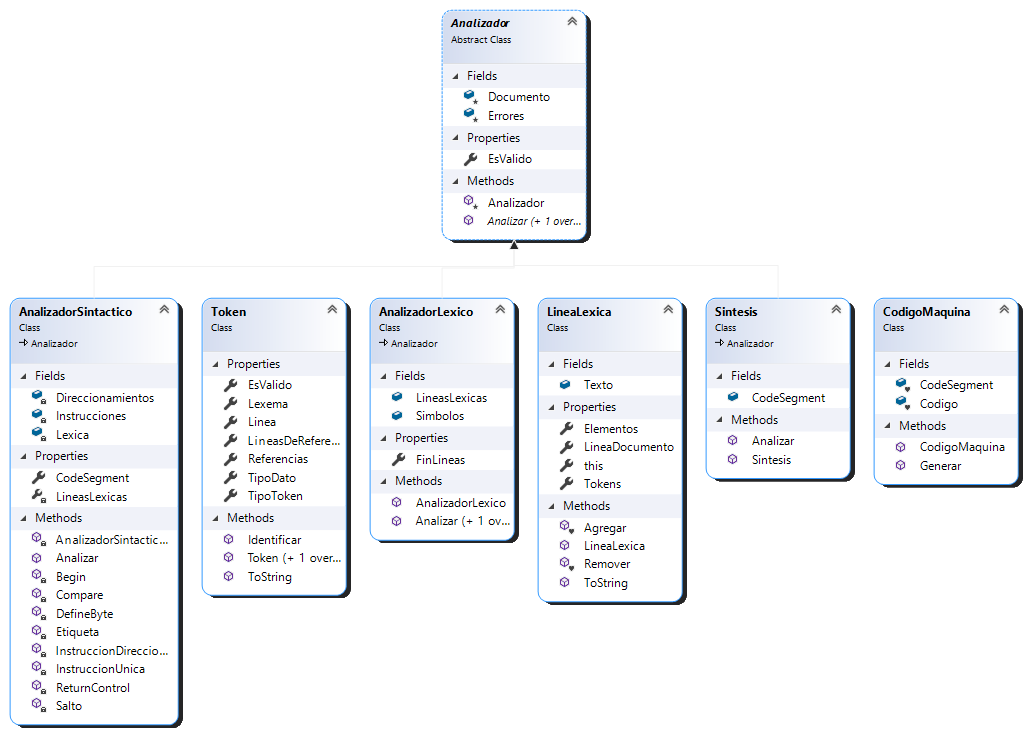
\includegraphics[width=\textwidth]{Compilador.png}
                \caption{Diagrama de clases de assambler/compilador de ensamblador.}
              \end{figure*}

\section{Ensamblador (Compilador)}
Se describen las fases del ensamblador:
\subsection{Analizador sintactico}
En esta primera etapa se clasifica cada palabra del código fuente en ensamblador en tokens, en caso de 
no identificar algún token el compilador envia el mensaje de "Sentencia no reconocida".
\subsection{Token}
Es la parte minima de cada instrucciones , las instrucciones están compuestas por uno ó varios token, como resultado del analisís anterior.
\subsection{Analizador léxico}
Valida que cada linea este escrita en un orden coherente y las clasifica en objetos del tipo "Lina léxica".
\subsection{Linea léxica}
Representa a una instrucción completa que ya ha sido,clasificada, validada y debidamente estructurada.
\subsection{Sintesís}
Fase de la compilación donde se extra información de todas las instrucciones en el programa preparandolas para su traducción final en binario.
Cabe destacar que esta etapa se realiza en dos fases debido a que en la primera se debe calcular la dirección de memoria de cada etiqueta para poder apuntar correctamente al segmento de memoria que contiene la instrucción de salto. 
\subsection{Código máquina}
Fase final donde se traduce el resultado de todas las etapas en un único archivo de código binario utilizando las definiciones de código de operación,Modificador y longuitud de instrucción.




\newpage
\section{Proceso de Ejecución}
Se obtiene la primera instrucción y se le da la
Unidad de Control. Para esto el Registro de
Instrucción (IR) deberá de tener la instrucción,
ya que es ahí donde la Unidad de Control la
busca.

La Unidad de Control se ayuda del
Analizador lexico para saber el tipo de instrucción
que ha recibido y el operando, y con ello
moverá datos a diferentes registros, y le dirá a
la ALU que haga una determinada operación.

Para finalizar, la Unidad de Control aumentara
a IP, el contador de programa, para poder
seguir con la siguiente instrucción, lo cual
devuelve al programa al paso 2 para procesar la
siguiente instrucción.

 El programa terminara cuando se ejecute la
última instrucción del programa.
\subsection{Clases del Programa}
Cada clase representa un componente diferente en el
microprocesador, y contiene sus métodos para cumplir
con la función.

\begin{itemize}
    \item Registros\\
    Almacena los registros de proposito general definidos en la arquitectura.
    \item Registro\\
    Abstracción de un registro de propostito general.\\
    Permite el acceso a la parte alta y baja de cada registro así como habilitar/deshabilitar la lectura y escritura de los mismos 
    \item CPU\\
    Unidad de control central\\
    Clase principal desde donde se llaman a todos los módulos para ejecutar cada una de las 
    instrucciones contenidas en la pila de instrucciones. 
    \item  Memoria \\
    Pila de instruciones y memoria del programador.\\
    Se almacenan el programa a ejecutar. 
    \item ALU    \\
    Aqui es donde se realizan las operaciones lógicas y aritméticas a nivel de bits. (Micro-código) 
    \item Banderas: 
    En esta clase se guarda el estado de las banderas durante la ejecución del código 
\end{itemize}

\newpage





\begin{figure*}[t]
    \section{Código de las clases principales}
\subsection{CPU}    
\begin{lstlisting}[language={[Sharp]C}, title={CPU}]
    public static class CPU
    {
        public static Alu.Alu Alu { get; private set; }
        public static Banderas Banderas { get; private set; }
        public static Memoria Memoria { get; private set; }
        static CPU()
        {
            CPU.Alu = new Alu.Alu();
            CPU.Banderas = new Banderas();
            CPU.Memoria = new Memoria();
            Reset();
        }
        public static void Reset()
        {
            CPU.Banderas.Clear();
            CPU.Memoria.Clear();
            Registros.Registros.Reset();
        }
        public static void Ejecutar(bool[] Operacion, bool[] Modificador,
         bool[] Operador1, bool[] Operador2){...}
    }
\end{lstlisting}
\end{figure*}
\newpage

\begin{figure*}[t]
\subsection{ALU}   
\begin{lstlisting}[language={[Sharp]C}, title={ALU}]
    public class Alu
    {   public const int Byte = 16;
        public bool[] Resultado = new bool[Byte * 2 + 1];
        public void ADD(bool[] Operador1, bool[] Operador2){ ... }  
        private bool HALF_ADD(bool A, bool B){ ... }  
        private bool FULL_ADD(bool A, bool B){ ... }  
        public void SUB(bool[] Operador1, bool[] Operador2){ ... }  
        public bool[] COMPLEMENTO_2(bool[] Operador1){ ... }  
        private bool AND(bool A, bool B){ ... }  
        public void AND(bool[] Operador1, bool[] Operador2){ ... }  
        public void OR(bool[] Operador1, bool[] Operador2){ ... }  
        public void NAND(bool[] Operador1, bool[] Operador2){ ... }  
        public void NOR(bool[] Operador1, bool[] Operador2){ ... }  
        public void MUL(bool[] Operador2){ ... }  
        public void NOT(bool[] Operador1){ ... }  
        private bool XOR(bool Operador1, bool Operador2){ ... }  
        public void XOR(bool[] Operador1, bool[] Operador2){ ... }  
        public void XNOR(bool[] Operador1, bool[] Operador2){ ... }  
        public void DIV(bool[] Divisor){ ... }         
    }
\end{lstlisting}
\end{figure*}

\newpage
\begin{figure*}[t]
    \subsection{Registros}
    \begin{lstlisting}[language={[Sharp]C}, title={Registros}]
    public static class Registros
    {
        public static Registro AX { get; private set; }
        public static Registro BX { get; private set; }
        public static Registro CX { get; private set; }
        public static Registro DX { get; private set; }
        public static Registro SI { get; private set; }
        public static Registro DI { get; private set; }
        public static Registro IP { get; private set; }
        public static Registro IA { get; private set; }
        public static Registro IR { get; private set; }
        static Registros()
        {
            Registros.AX = new Registro("AX");
            Registros.BX = new Registro("BX");
            Registros.CX = new Registro("CX");
            Registros.DX = new Registro("DX");
            Registros.SI = new Registro("SI");
            Registros.DI = new Registro("DI");
            Registros.IP = new Registro("IP");
            Registros.IA = new Registro("IA");
            Registros.IR = new Registro("IR");
        }
        internal static void Reset()
        {
            Registros.AX.Clear();
            Registros.BX.Clear();
            Registros.CX.Clear();
            Registros.DX.Clear();
            Registros.SI.Clear();
            Registros.DI.Clear();
            Registros.IP.Clear();
        }
    }
\end{lstlisting}
\end{figure*}
\newpage

\begin{figure*}[t]
    \subsection{Registro}
\begin{lstlisting}[language={[Sharp]C}, title={Registro}]
    public class Registro : Localidad
    {
        public string Nombre { get; private set; }
        private ParteRegistro High;
        public ParteRegistro Low;
        public void SetHigh(bool[] High){ ... }
        public void SetLow(bool[] Low){ ... }
    }
\end{lstlisting}
\end{figure*}

\newpage


\begin{figure*}[t]
    \subsection{Memoria}
\begin{lstlisting}[language={[Sharp]C}, title={Memoria}]
    public class Memoria 
    {
        public bool[] this[bool[] direccion]
        {
            set
            {
                Escribir(direccion, value);
            }
        }
        private ObservableCollection<Celda> Real;

        public void Cargar(string CodigoMaquina) { ... }
        public void Cargar(bool[][] programa) { ... }
        public static bool[] CalcularDireccion(bool[] Numero) { ... }
        internal void Clear() { ... }
        public bool[] Leer(bool[] direccion) { ... }
        public void Escribir(bool[] direccion, bool[] Valor){ ... }
    }
\end{lstlisting}
\end{figure*}
\newpage

\begin{figure*}[t]
    \subsection{Banderas}
\begin{lstlisting}[language={[Sharp]C}, title={Banderas}]
    public class Banderas :
    {
        private bool Carry;    
        private bool Signo;   
        private bool Zero;
        private bool OverFlow;
        internal void Clear()
        {
            Carry = false;
            Signo = false;
            Zero = false;
            OverFlow = false;
        }
    }
\end{lstlisting}
\end{figure*}

\end{document}
